\documentclass{beamer}
\usetheme{Luebeck}
\usecolortheme{seahorse}
\usefonttheme{structurebold,serif}
\setbeamertemplate{navigation symbols}{\usebeamerfont{footline}\insertframenumber/\inserttotalframenumber}
\setlength{\parskip}{\bigskipamount}
\usepackage{luatexja-fontspec}
\setmainfont{STIX Two Text}
\setsansfont{Helvetica}
\setmonofont{Inconsolata}
\setmainjfont{YuKyo_Yoko-Medium}[BoldFont=YuKyo_Yoko-Bold]
\setsansjfont{YuGo-Medium}[BoldFont=YuGo-Bold]
\usepackage{mathtools}
\usepackage[warnings-off={mathtools-colon,mathtools-overbracket}]{unicode-math}
\unimathsetup{math-style=ISO,bold-style=ISO}
\setmathfont{STIX Two Math}
\mathtoolsset{showonlyrefs=true}
\usepackage{subcaption}
\usepackage{multimedia}
\usepackage{tikz}
\def\lpiece{-- ([turn]180:1) -- ([turn]-120:1) -- ([turn]-75:0.707) -- cycle}
\def\spiece{-- ([turn]180:1) -- ([turn]-150:1) -- cycle}
\def\dred{\draw[red,very thick]}
\def\dfil{\filldraw[fill=lightgray]}

\title{パズルキューブSquare-1の紹介}
\author{宇佐見 公輔}
\date{2024年2月25日}
\begin{document}
\maketitle

\begin{frame}
    \frametitle{きっかけ}

    昨年末に、立体パズルの専門店TORIBOの福袋を買いました。

    \begin{figure}
        \centering
        \caption{福袋に入っていたカレンダーキューブ}
        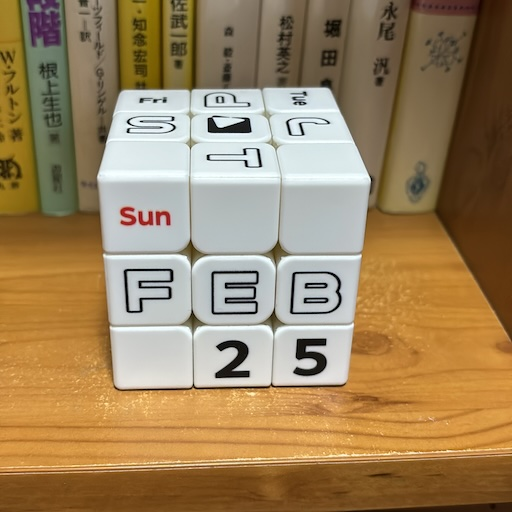
\includegraphics[width=0.40\columnwidth,height=0.40\columnwidth]{images/calendar.jpg}
    \end{figure}

    その中に入っていたパズルのひとつ、Square-1が結構楽しくて今ハマっているので紹介します。
\end{frame}

\begin{frame}
    \frametitle{Square-1とは}

    Square-1(スクエアワン)は、ルービックキューブのような立体パズルです。

    \begin{figure}
        \centering
        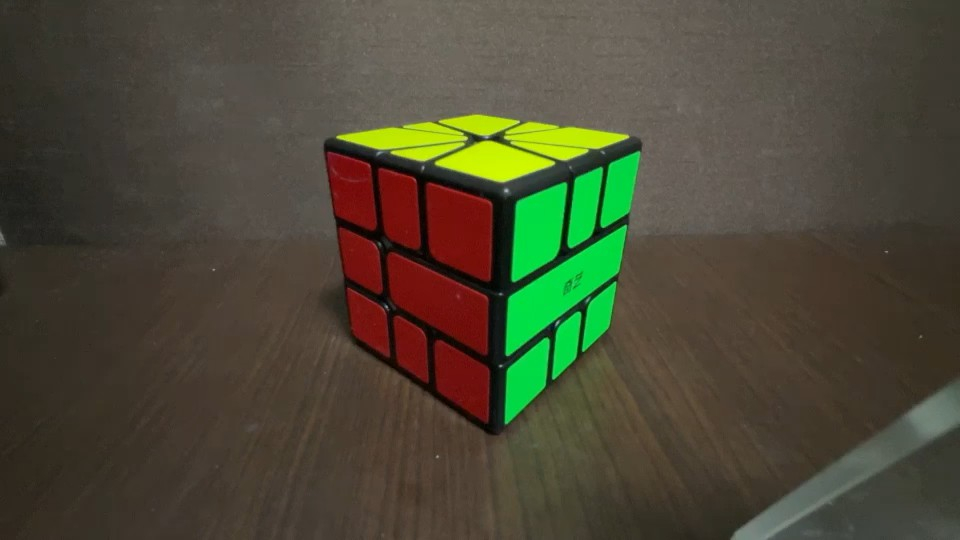
\includegraphics[width=0.96\columnwidth,height=0.54\columnwidth]{images/square-1.jpg}
    \end{figure}
\end{frame}

\begin{frame}
    \frametitle{水平方向の回転}

    \begin{figure}
        \centering
        %\movie{
        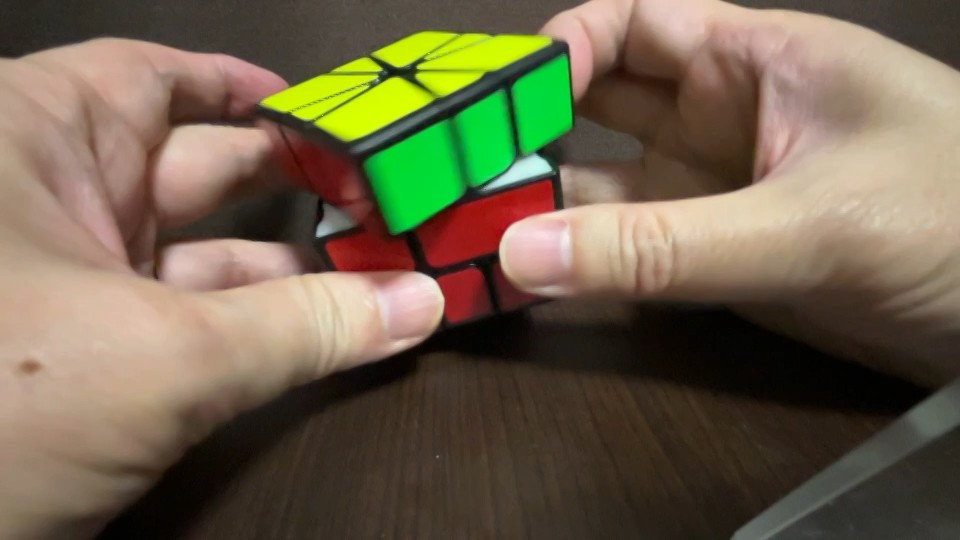
\includegraphics[width=0.96\columnwidth,height=0.54\columnwidth]{images/horizontal.jpg}
        %}{videos/horizontal.mov}
    \end{figure}
\end{frame}

\begin{frame}
    \frametitle{垂直方向の回転(twist操作)}

    \begin{figure}
        \centering
        %\movie{
        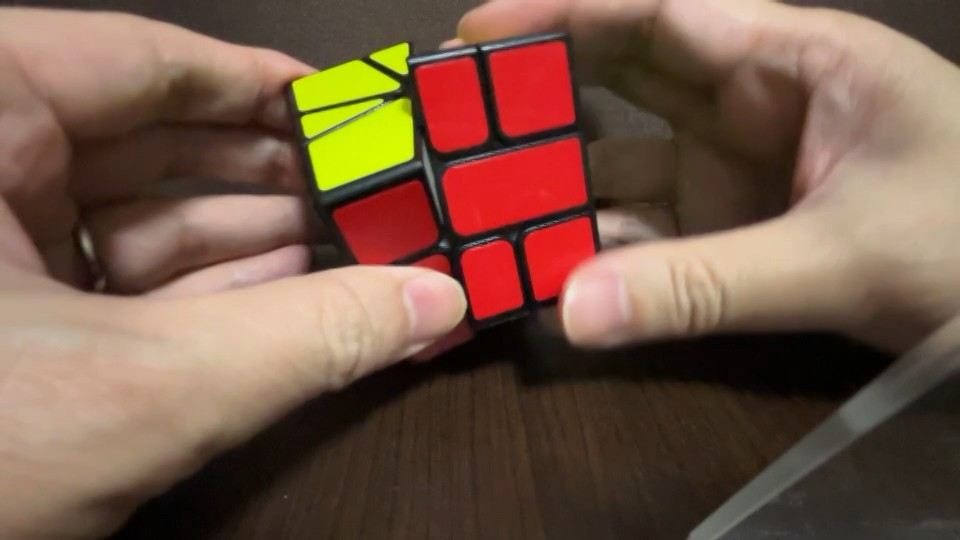
\includegraphics[width=0.96\columnwidth,height=0.54\columnwidth]{images/vertical.jpg}
        %}{videos/vertical.mov}
    \end{figure}
\end{frame}

\begin{frame}
    \frametitle{ピースの形状}

    上層と下層は、それぞれ8個のピースで構成されています。
    中心角が60度の大ピースが4個、30度の小ピースが4個です。

    \begin{figure}
        \centering
        \begin{subfigure}{0.40\columnwidth}
            \centering
            \caption{上層と下層}
            \begin{tikzpicture}[scale=1.8]
                \draw (-15:1) \spiece;
                \draw ( 15:1) \lpiece;
                \draw ( 75:1) \spiece;
                \draw (105:1) \lpiece;
                \draw (165:1) \spiece;
                \draw (195:1) \lpiece;
                \draw (255:1) \spiece;
                \draw (285:1) \lpiece;
            \end{tikzpicture}
        \end{subfigure}
        \begin{subfigure}{0.40\columnwidth}
            \centering
            \caption{中層}
            \begin{tikzpicture}[scale=1.8]
                \draw ( 75:1) -- (135:1.366) -- (225:1.366) -- (255:1) -- cycle;
                \draw (255:1) -- (315:1.366) -- ( 45:1.366) -- ( 75:1) -- cycle;
            \end{tikzpicture}
        \end{subfigure}
    \end{figure}

    中層は、2個のピースで構成されています。
    正方形を斜めに切った形で、上層や下層のピースの切れ目と重なっています。
\end{frame}

\begin{frame}
    \frametitle{WCAの認定競技}

    WCA(World Cube Association、世界キューブ協会)は、ルービックキューブの世界大会を開催しています。

    ルービックキューブ以外の立体回転パズルも認定しており、Square-1もそのひとつです。

    WCAの認定競技に使われるパズル:
    \begin{itemize}
        \item 2×2×2、3×3×3、4×4×4、5×5×5、6×6×6、7×7×7
        \item メガミンクス
        \item ピラミンクス
        \item スキューブ
        \item Square-1
        \item クロック
    \end{itemize}
\end{frame}

\begin{frame}
    \frametitle{WCA世界記録}

    スピード競技の世界記録を比べると、立体パズルのおおまかな難易度が見えてきます。

    \begin{itemize}
        \item 2×2×2:0.43秒
        \item 3×3×3:3.13秒
        \item 4×4×4:16.79秒
        \item 5×5×5:32.60秒
        \item Square-1:3.69秒
    \end{itemize}

    Square-1の難易度は、通常の3×3×3のルービックキューブに近いと言えそうです。
\end{frame}

\begin{frame}
    \frametitle{余談:スピード競技とは何か}

    立体パズルのスピード競技は何を競っているのでしょうか?

    指先の器用さでしょうか? それよりも、次のことが重要です。

    \begin{itemize}
        \item 最善を求める日頃の研究
        \item その研究を時間内に素早く引き出して実行する能力
    \end{itemize}

    つまり、頭脳競技という側面が強いと言えます。

    ※僕自身はスピード競技のプレイヤーではないので、参考程度に。
\end{frame}

\begin{frame}
    \frametitle{Square-1パズルの解き方}

    よく使われている解法の流れは次のとおりです。

    \begin{itemize}
        \item Step 1:上層と下層を正方形に戻す。
        \item Step 2:上層と下層の各ピースを正しい位置に戻す。
        \item Step 3:中層を正方形に戻す。
    \end{itemize}

    Step 1の手順がある点に、立方体以外の形になるというSquare-1の特徴が強くあらわれています。

    Step 2の正方形に戻したあとの手順も、いろいろな手法があって工夫の余地が多く、興味深いところです。

    Step 3で中層が出てきますが、中層の状態は2種類しかなく、垂直方向の回転の回数が偶数回か奇数回かだけで決まります。
\end{frame}

\begin{frame}
    \frametitle{正方形以外にどんな形ができるか}

    上層と下層の形状について探ってみます。

    正方形になっている場合は、大ピースがコーナー、小ピースがエッジになっています。

    \begin{figure}
        \centering
        \begin{subfigure}{0.40\columnwidth}
            \begin{tikzpicture}[scale=0.9]
                \draw (-15:1) \spiece;
                \draw ( 15:1) \lpiece;
                \draw ( 75:1) \spiece;
                \draw (105:1) \lpiece;
                \draw (165:1) \spiece;
                \draw (195:1) \lpiece;
                \draw (255:1) \spiece;
                \draw (285:1) \lpiece;
            \end{tikzpicture}
        \end{subfigure}
        \begin{subfigure}{0.40\columnwidth}
            \begin{tikzpicture}[scale=0.9]
                \draw (-15:1) \lpiece;
                \draw ( 45:1) \lpiece;
                \draw (105:1) \spiece;
                \draw (135:1) \spiece;
                \draw (165:1) \spiece;
                \draw (195:1) \lpiece;
                \draw (255:1) \spiece;
                \draw (285:1) \lpiece;
            \end{tikzpicture}
        \end{subfigure}
    \end{figure}

    しかし正方形以外の形では、そういった単純な関係にはなりません。
    また、大ピースが4つであるとも限りません。最大では6つ(小ピースなし)、最小では2つ(小ピース8つ)になります。
\end{frame}

\begin{frame}
    \frametitle{上層・下層の取りうる形状(1)}

    \begin{figure}
        \centering
        \caption{大ピース6}
        \begin{subfigure}{0.28\columnwidth}
            \centering
            \begin{tikzpicture}[scale=0.9]
                \draw (-90:1) \lpiece;
                \draw (-30:1) \lpiece;
                \draw ( 30:1) \lpiece;
                \draw ( 90:1) \lpiece;
                \draw (150:1) \lpiece;
                \draw (210:1) \lpiece;
            \end{tikzpicture}
        \end{subfigure}
    \end{figure}

    \begin{figure}
        \centering
        \caption{大ピース5+小ピース2}
        \begin{subfigure}{0.28\columnwidth}
            \centering
            \begin{tikzpicture}[scale=0.9]
                \dred (-90:1) \spiece;
                \dred (-60:1) \spiece;
                \draw (-30:1) \lpiece;
                \draw ( 30:1) \lpiece;
                \draw ( 90:1) \lpiece;
                \draw (150:1) \lpiece;
                \draw (210:1) \lpiece;
            \end{tikzpicture}
        \end{subfigure}
        \begin{subfigure}{0.28\columnwidth}
            \centering
            \begin{tikzpicture}[scale=0.9]
                \dred (-90:1) \spiece;
                \draw (-60:1) \lpiece;
                \dred (  0:1) \spiece;
                \draw ( 30:1) \lpiece;
                \draw ( 90:1) \lpiece;
                \draw (150:1) \lpiece;
                \draw (210:1) \lpiece;
            \end{tikzpicture}
        \end{subfigure}
        \begin{subfigure}{0.28\columnwidth}
            \centering
            \begin{tikzpicture}[scale=0.9]
                \dred (-90:1) \spiece;
                \draw (-60:1) \lpiece;
                \draw (  0:1) \lpiece;
                \dred ( 60:1) \spiece;
                \draw ( 90:1) \lpiece;
                \draw (150:1) \lpiece;
                \draw (210:1) \lpiece;
            \end{tikzpicture}
        \end{subfigure}
    \end{figure}

    ※図が見やすいように、小ピースを赤くしています。
\end{frame}

\begin{frame}
    \frametitle{上層・下層の取りうる形状(2)}

    \begin{figure}
        \centering
        \caption{大ピース4+小ピース4}
        % Square
        \begin{subfigure}{0.18\columnwidth}
            \centering
            \begin{tikzpicture}[scale=0.7]
                \dred (-90:1) \spiece;
                \draw (-60:1) \lpiece;
                \dred (  0:1) \spiece;
                \draw ( 30:1) \lpiece;
                \dred ( 90:1) \spiece;
                \draw (120:1) \lpiece;
                \dred (180:1) \spiece;
                \draw (210:1) \lpiece;
            \end{tikzpicture}
        \end{subfigure}
        % Kite
        \begin{subfigure}{0.18\columnwidth}
            \centering
            \begin{tikzpicture}[scale=0.7]
                \draw (-90:1) \lpiece;
                \dred (-30:1) \spiece;
                \draw (  0:1) \lpiece;
                \dred ( 60:1) \spiece;
                \dred ( 90:1) \spiece;
                \draw (120:1) \lpiece;
                \dred (180:1) \spiece;
                \draw (210:1) \lpiece;
            \end{tikzpicture}
        \end{subfigure}
        % Barrel
        \begin{subfigure}{0.18\columnwidth}
            \centering
            \begin{tikzpicture}[scale=0.7]
                \dred (-90:1) \spiece;
                \dred (-60:1) \spiece;
                \draw (-30:1) \lpiece;
                \draw ( 30:1) \lpiece;
                \dred ( 90:1) \spiece;
                \dred (120:1) \spiece;
                \draw (150:1) \lpiece;
                \draw (210:1) \lpiece;
            \end{tikzpicture}
        \end{subfigure}
        % Scallop
        \begin{subfigure}{0.18\columnwidth}
            \centering
            \begin{tikzpicture}[scale=0.7]
                \draw (-90:1) \lpiece;
                \draw (-30:1) \lpiece;
                \dred ( 30:1) \spiece;
                \dred ( 60:1) \spiece;
                \dred ( 90:1) \spiece;
                \dred (120:1) \spiece;
                \draw (150:1) \lpiece;
                \draw (210:1) \lpiece;
            \end{tikzpicture}
        \end{subfigure}
        % Shield
        \begin{subfigure}{0.18\columnwidth}
            \centering
            \begin{tikzpicture}[scale=0.7]
                \dred (-90:1) \spiece;
                \dred (-60:1) \spiece;
                \draw (-30:1) \lpiece;
                \dred ( 30:1) \spiece;
                \dred ( 60:1) \spiece;
                \draw ( 90:1) \lpiece;
                \draw (150:1) \lpiece;
                \draw (210:1) \lpiece;
            \end{tikzpicture}
        \end{subfigure}
        % Left Paw
        \begin{subfigure}{0.18\columnwidth}
            \centering
            \begin{tikzpicture}[scale=0.7]
                \dred (-90:1) \spiece;
                \draw (-60:1) \lpiece;
                \dred (  0:1) \spiece;
                \draw ( 30:1) \lpiece;
                \draw ( 90:1) \lpiece;
                \draw (150:1) \lpiece;
                \dred (210:1) \spiece;
                \dred (240:1) \spiece;
            \end{tikzpicture}
        \end{subfigure}
        % Right Paw
        \begin{subfigure}{0.18\columnwidth}
            \centering
            \begin{tikzpicture}[scale=0.7]
                \dred (-90:1) \spiece;
                \dred (-60:1) \spiece;
                \draw (-30:1) \lpiece;
                \draw ( 30:1) \lpiece;
                \draw ( 90:1) \lpiece;
                \dred (150:1) \spiece;
                \draw (180:1) \lpiece;
                \dred (240:1) \spiece;
            \end{tikzpicture}
        \end{subfigure}
        % Left Fist
        \begin{subfigure}{0.18\columnwidth}
            \centering
            \begin{tikzpicture}[scale=0.7]
                \dred (-90:1) \spiece;
                \draw (-60:1) \lpiece;
                \draw (  0:1) \lpiece;
                \dred ( 60:1) \spiece;
                \dred ( 90:1) \spiece;
                \draw (120:1) \lpiece;
                \dred (180:1) \spiece;
                \draw (210:1) \lpiece;
            \end{tikzpicture}
        \end{subfigure}
        % Right Fist
        \begin{subfigure}{0.18\columnwidth}
            \centering
            \begin{tikzpicture}[scale=0.7]
                \draw (-90:1) \lpiece;
                \dred (-30:1) \spiece;
                \draw (  0:1) \lpiece;
                \dred ( 60:1) \spiece;
                \dred ( 90:1) \spiece;
                \draw (120:1) \lpiece;
                \draw (180:1) \lpiece;
                \dred (240:1) \spiece;
            \end{tikzpicture}
        \end{subfigure}
        % Mushroom
        \begin{subfigure}{0.18\columnwidth}
            \centering
            \begin{tikzpicture}[scale=0.7]
                \draw (-90:1) \lpiece;
                \draw (-30:1) \lpiece;
                \dred ( 30:1) \spiece;
                \dred ( 60:1) \spiece;
                \dred ( 90:1) \spiece;
                \draw (120:1) \lpiece;
                \draw (180:1) \lpiece;
                \dred (240:1) \spiece;
            \end{tikzpicture}
        \end{subfigure}
    \end{figure}

    ※回転で重なれば同じ形、鏡映は異なる形とします。
\end{frame}

\begin{frame}
    \frametitle{上層・下層の取りうる形状(3)}

    \begin{figure}
        \centering
        \caption{大ピース3+小ピース6}
        \begin{subfigure}{0.18\columnwidth}
            \centering
            \begin{tikzpicture}[scale=0.7]
                \draw (-90:1) \lpiece;
                \dred (-30:1) \spiece;
                \dred (  0:1) \spiece;
                \dred ( 30:1) \spiece;
                \dred ( 60:1) \spiece;
                \dred ( 90:1) \spiece;
                \dred (120:1) \spiece;
                \draw (150:1) \lpiece;
                \draw (210:1) \lpiece;
            \end{tikzpicture}
        \end{subfigure}
        \begin{subfigure}{0.18\columnwidth}
            \centering
            \begin{tikzpicture}[scale=0.7]
                \draw (-90:1) \lpiece;
                \dred (-30:1) \spiece;
                \dred (  0:1) \spiece;
                \dred ( 30:1) \spiece;
                \dred ( 60:1) \spiece;
                \dred ( 90:1) \spiece;
                \draw (120:1) \lpiece;
                \dred (180:1) \spiece;
                \draw (210:1) \lpiece;
            \end{tikzpicture}
        \end{subfigure}
        \begin{subfigure}{0.18\columnwidth}
            \centering
            \begin{tikzpicture}[scale=0.7]
                \draw (-90:1) \lpiece;
                \dred (-30:1) \spiece;
                \draw (  0:1) \lpiece;
                \dred ( 60:1) \spiece;
                \dred ( 90:1) \spiece;
                \dred (120:1) \spiece;
                \dred (150:1) \spiece;
                \dred (180:1) \spiece;
                \draw (210:1) \lpiece;
            \end{tikzpicture}
        \end{subfigure}
        \begin{subfigure}{0.18\columnwidth}
            \centering
            \begin{tikzpicture}[scale=0.7]
                \draw (-90:1) \lpiece;
                \dred (-30:1) \spiece;
                \dred (  0:1) \spiece;
                \dred ( 30:1) \spiece;
                \dred ( 60:1) \spiece;
                \draw ( 90:1) \lpiece;
                \dred (150:1) \spiece;
                \dred (180:1) \spiece;
                \draw (210:1) \lpiece;
            \end{tikzpicture}
        \end{subfigure}
        \begin{subfigure}{0.18\columnwidth}
            \centering
            \begin{tikzpicture}[scale=0.7]
                \draw (-90:1) \lpiece;
                \dred (-30:1) \spiece;
                \dred (  0:1) \spiece;
                \draw ( 30:1) \lpiece;
                \dred ( 90:1) \spiece;
                \dred (120:1) \spiece;
                \dred (150:1) \spiece;
                \dred (180:1) \spiece;
                \draw (210:1) \lpiece;
            \end{tikzpicture}
        \end{subfigure}
        \begin{subfigure}{0.18\columnwidth}
            \centering
            \begin{tikzpicture}[scale=0.7]
                \dred (-90:1) \spiece;
                \dred (-60:1) \spiece;
                \dred (-30:1) \spiece;
                \dred (  0:1) \spiece;
                \draw ( 30:1) \lpiece;
                \dred ( 90:1) \spiece;
                \draw (120:1) \lpiece;
                \dred (180:1) \spiece;
                \draw (210:1) \lpiece;
            \end{tikzpicture}
        \end{subfigure}
        \begin{subfigure}{0.18\columnwidth}
            \centering
            \begin{tikzpicture}[scale=0.7]
                \dred (-90:1) \spiece;
                \dred (-60:1) \spiece;
                \dred (-30:1) \spiece;
                \draw (  0:1) \lpiece;
                \dred ( 60:1) \spiece;
                \dred ( 90:1) \spiece;
                \draw (120:1) \lpiece;
                \dred (180:1) \spiece;
                \draw (210:1) \lpiece;
            \end{tikzpicture}
        \end{subfigure}
        \begin{subfigure}{0.18\columnwidth}
            \centering
            \begin{tikzpicture}[scale=0.7]
                \draw (-90:1) \lpiece;
                \dred (-30:1) \spiece;
                \draw (  0:1) \lpiece;
                \dred ( 60:1) \spiece;
                \dred ( 90:1) \spiece;
                \draw (120:1) \lpiece;
                \dred (180:1) \spiece;
                \dred (210:1) \spiece;
                \dred (240:1) \spiece;
            \end{tikzpicture}
        \end{subfigure}
        \begin{subfigure}{0.18\columnwidth}
            \centering
            \begin{tikzpicture}[scale=0.7]
                \dred (-90:1) \spiece;
                \dred (-60:1) \spiece;
                \draw (-30:1) \lpiece;
                \dred ( 30:1) \spiece;
                \dred ( 60:1) \spiece;
                \draw ( 90:1) \lpiece;
                \dred (150:1) \spiece;
                \dred (180:1) \spiece;
                \draw (210:1) \lpiece;
            \end{tikzpicture}
        \end{subfigure}
        \begin{subfigure}{0.18\columnwidth}
            \centering
            \begin{tikzpicture}[scale=0.7]
                \dred (-90:1) \spiece;
                \dred (-60:1) \spiece;
                \dred (-30:1) \spiece;
                \draw (  0:1) \lpiece;
                \dred ( 60:1) \spiece;
                \dred ( 90:1) \spiece;
                \dred (120:1) \spiece;
                \draw (150:1) \lpiece;
                \draw (210:1) \lpiece;
            \end{tikzpicture}
        \end{subfigure}
    \end{figure}

    \begin{figure}
        \centering
        \caption{大ピース2+小ピース8}
        % 8
        \begin{subfigure}{0.18\columnwidth}
            \centering
            \begin{tikzpicture}[scale=0.7]
                \draw (-90:1) \lpiece;
                \dred (-30:1) \spiece;
                \dred (  0:1) \spiece;
                \dred ( 30:1) \spiece;
                \dred ( 60:1) \spiece;
                \dred ( 90:1) \spiece;
                \dred (120:1) \spiece;
                \dred (150:1) \spiece;
                \dred (180:1) \spiece;
                \draw (210:1) \lpiece;
            \end{tikzpicture}
        \end{subfigure}
        % 7-1
        \begin{subfigure}{0.18\columnwidth}
            \centering
            \begin{tikzpicture}[scale=0.7]
                \draw (-90:1) \lpiece;
                \dred (-30:1) \spiece;
                \dred (  0:1) \spiece;
                \dred ( 30:1) \spiece;
                \dred ( 60:1) \spiece;
                \dred ( 90:1) \spiece;
                \dred (120:1) \spiece;
                \dred (150:1) \spiece;
                \draw (180:1) \lpiece;
                \dred (240:1) \spiece;
            \end{tikzpicture}
        \end{subfigure}
        % 6-2
        \begin{subfigure}{0.18\columnwidth}
            \centering
            \begin{tikzpicture}[scale=0.7]
                \draw (-90:1) \lpiece;
                \dred (-30:1) \spiece;
                \dred (  0:1) \spiece;
                \dred ( 30:1) \spiece;
                \dred ( 60:1) \spiece;
                \dred ( 90:1) \spiece;
                \dred (120:1) \spiece;
                \draw (150:1) \lpiece;
                \dred (210:1) \spiece;
                \dred (240:1) \spiece;
            \end{tikzpicture}
        \end{subfigure}
        % 5-3
        \begin{subfigure}{0.18\columnwidth}
            \centering
            \begin{tikzpicture}[scale=0.7]
                \draw (-90:1) \lpiece;
                \dred (-30:1) \spiece;
                \dred (  0:1) \spiece;
                \dred ( 30:1) \spiece;
                \dred ( 60:1) \spiece;
                \dred ( 90:1) \spiece;
                \draw (120:1) \lpiece;
                \dred (180:1) \spiece;
                \dred (210:1) \spiece;
                \dred (240:1) \spiece;
            \end{tikzpicture}
        \end{subfigure}
        % 4-4
        \begin{subfigure}{0.18\columnwidth}
            \centering
            \begin{tikzpicture}[scale=0.7]
                \draw (-90:1) \lpiece;
                \dred (-30:1) \spiece;
                \dred (  0:1) \spiece;
                \dred ( 30:1) \spiece;
                \dred ( 60:1) \spiece;
                \draw ( 90:1) \lpiece;
                \dred (150:1) \spiece;
                \dred (180:1) \spiece;
                \dred (210:1) \spiece;
                \dred (240:1) \spiece;
            \end{tikzpicture}
        \end{subfigure}
    \end{figure}
\end{frame}

\begin{frame}
    \frametitle{上層と下層の組み合わせ}

    上層と下層とで大ピースの合計が8つになるような組み合わせがありえます。

    \begin{figure}
        \centering
        \begin{subfigure}{0.30\columnwidth}
            \begin{tikzpicture}[scale=0.8]
                \begin{scope}[shift={(0,0)}]
                    \draw[dashed] (0,1.5) -- (0,-1.5);
                    \draw (-90:1) \spiece;
                    \draw (-60:1) \lpiece;
                    \draw (  0:1) \spiece;
                    \draw ( 30:1) \lpiece;
                    \draw ( 90:1) \spiece;
                    \draw (120:1) \lpiece;
                    \draw (180:1) \spiece;
                    \draw (210:1) \lpiece;
                \end{scope}
                \begin{scope}[shift={(0,-3)}]
                    \draw[dashed] (0,1.5) -- (0,-1.5);
                    \draw (-90:1) \lpiece;
                    \draw (-30:1) \spiece;
                    \draw (  0:1) \lpiece;
                    \draw ( 60:1) \spiece;
                    \draw ( 90:1) \lpiece;
                    \draw (150:1) \spiece;
                    \draw (180:1) \lpiece;
                    \draw (240:1) \spiece;
                \end{scope}
            \end{tikzpicture}
        \end{subfigure}
        \begin{subfigure}{0.30\columnwidth}
            \begin{tikzpicture}[scale=0.8]
                \begin{scope}[shift={(0,0)}]
                    \draw[dashed] (0,1.5) -- (0,-1.5);
                    \draw (-90:1) \spiece;
                    \draw (-60:1) \spiece;
                    \draw (-30:1) \spiece;
                    \draw (  0:1) \spiece;
                    \draw ( 30:1) \lpiece;
                    \draw ( 90:1) \lpiece;
                    \draw (150:1) \spiece;
                    \draw (180:1) \spiece;
                    \draw (210:1) \lpiece;
                \end{scope}
                \begin{scope}[shift={(0,-3)}]
                    \draw[dashed] (0,1.5) -- (0,-1.5);
                    \draw (-90:1) \lpiece;
                    \draw (-30:1) \spiece;
                    \draw (  0:1) \lpiece;
                    \draw ( 60:1) \spiece;
                    \draw ( 90:1) \lpiece;
                    \draw (150:1) \lpiece;
                    \draw (210:1) \lpiece;
                \end{scope}
            \end{tikzpicture}
        \end{subfigure}
        \begin{subfigure}{0.30\columnwidth}
            \begin{tikzpicture}[scale=0.8]
                \begin{scope}
                    \draw[dashed] (0,1.5) -- (0,-1.5);
                    \draw (-90:1) \spiece;
                    \draw (-60:1) \spiece;
                    \draw (-30:1) \lpiece;
                    \draw ( 30:1) \spiece;
                    \draw ( 60:1) \spiece;
                    \draw ( 90:1) \spiece;
                    \draw (120:1) \lpiece;
                    \draw (180:1) \spiece;
                    \draw (210:1) \spiece;
                    \draw (240:1) \spiece;
                \end{scope}
                \begin{scope}[shift={(0,-3)}]
                    \draw[dashed] (0,1.5) -- (0,-1.5);
                    \draw (-90:1) \lpiece;
                    \draw (-30:1) \lpiece;
                    \draw ( 30:1) \lpiece;
                    \draw ( 90:1) \lpiece;
                    \draw (150:1) \lpiece;
                    \draw (210:1) \lpiece;
                \end{scope}
            \end{tikzpicture}
        \end{subfigure}
    \end{figure}

    ※上層は上から、下層は下から見た図です。
\end{frame}

\begin{frame}
    \frametitle{twist操作による状態の変化}

    twist操作は、上層の半分と下層の半分を入れ替える操作です。

    \begin{figure}
        \centering
        \begin{tikzpicture}[scale=0.8]
            \begin{scope}[shift={(0,0)}]
                \draw[dashed] (0,1.5) -- (0,-1.5);
                \draw (-90:1) \spiece;
                \draw (-60:1) \lpiece;
                \draw (  0:1) \spiece;
                \draw ( 30:1) \lpiece;
                \draw ( 90:1) \spiece;
                \draw (120:1) \lpiece;
                \draw (180:1) \spiece;
                \draw (210:1) \lpiece;
            \end{scope}
            \begin{scope}[shift={(0,-3)}]
                \draw[dashed] (0,1.5) -- (0,-1.5);
                \dfil (-90:1) \lpiece;
                \dfil (-30:1) \spiece;
                \dfil (  0:1) \lpiece;
                \dfil ( 60:1) \spiece;
                \dfil ( 90:1) \lpiece;
                \dfil (150:1) \spiece;
                \dfil (180:1) \lpiece;
                \dfil (240:1) \spiece;
            \end{scope}
            \begin{scope}[shift={(3.8,0)}]
                \draw[->] (-2.4,-1.5) -- node[above]{twist} (-1.4,-1.5);
                \draw[dashed] (0,1.5) -- (0,-1.5);
                \dfil (-90:1) \lpiece;
                \dfil (-30:1) \spiece;
                \dfil (  0:1) \lpiece;
                \dfil ( 60:1) \spiece;
                \draw ( 90:1) \spiece;
                \draw (120:1) \lpiece;
                \draw (180:1) \spiece;
                \draw (210:1) \lpiece;
            \end{scope}
            \begin{scope}[shift={(3.8,-3)}]
                \draw[dashed] (0,1.5) -- (0,-1.5);
                \draw (-90:1) \spiece;
                \draw (-60:1) \lpiece;
                \draw (  0:1) \spiece;
                \draw ( 30:1) \lpiece;
                \dfil ( 90:1) \lpiece;
                \dfil (150:1) \spiece;
                \dfil (180:1) \lpiece;
                \dfil (240:1) \spiece;
            \end{scope}
        \end{tikzpicture}
    \end{figure}

    ※上層は上から、下層は下から見た図です。
\end{frame}

\begin{frame}
    \frametitle{正方形を作る手順(1)}

    正方形を作る手順は、正方形から逆算して考えると良いです。

    \begin{figure}
        \centering
        \begin{tikzpicture}[scale=0.8]
            \begin{scope}[shift={(0,0)}]
                \draw[dashed] (0,1.5) -- (0,-1.5);
                \draw (-90:1) \spiece;
                \draw (-60:1) \lpiece;
                \draw (  0:1) \lpiece;
                \draw ( 60:1) \spiece;
                \draw ( 90:1) \spiece;
                \draw (120:1) \lpiece;
                \draw (180:1) \lpiece;
                \draw (240:1) \spiece;
            \end{scope}
            \begin{scope}[shift={(0,-3)}]
                \draw[dashed] (0,1.5) -- (0,-1.5);
                \draw (-90:1) \lpiece;
                \draw (-30:1) \spiece;
                \draw (  0:1) \spiece;
                \draw ( 30:1) \lpiece;
                \draw ( 90:1) \lpiece;
                \draw (150:1) \spiece;
                \draw (180:1) \spiece;
                \draw (210:1) \lpiece;
            \end{scope}
            \begin{scope}[shift={(3.8,0)}]
                \draw[->] (-2.4,-1.5) -- (-1.4,-1.5);
                \draw[dashed] (0,1.5) -- (0,-1.5);
                \draw (-90:1) \lpiece;
                \draw (-30:1) \spiece;
                \draw (  0:1) \lpiece;
                \draw ( 60:1) \spiece;
                \draw ( 90:1) \spiece;
                \draw (120:1) \lpiece;
                \draw (180:1) \spiece;
                \draw (210:1) \lpiece;
            \end{scope}
            \begin{scope}[shift={(3.8,-3)}]
                \draw[dashed] (0,1.5) -- (0,-1.5);
                \draw (-90:1) \spiece;
                \draw (-60:1) \lpiece;
                \draw (  0:1) \spiece;
                \draw ( 30:1) \lpiece;
                \draw ( 90:1) \lpiece;
                \draw (150:1) \spiece;
                \draw (180:1) \lpiece;
                \draw (240:1) \spiece;
            \end{scope}
            \begin{scope}[shift={(7.6,0)}]
                \draw[->] (-2.4,-1.5) -- (-1.4,-1.5);
                \draw[dashed] (0,1.5) -- (0,-1.5);
                \draw (-90:1) \spiece;
                \draw (-60:1) \lpiece;
                \draw (  0:1) \spiece;
                \draw ( 30:1) \lpiece;
                \draw ( 90:1) \spiece;
                \draw (120:1) \lpiece;
                \draw (180:1) \spiece;
                \draw (210:1) \lpiece;
            \end{scope}
            \begin{scope}[shift={(7.6,-3)}]
                \draw[dashed] (0,1.5) -- (0,-1.5);
                \draw (-90:1) \lpiece;
                \draw (-30:1) \spiece;
                \draw (  0:1) \lpiece;
                \draw ( 60:1) \spiece;
                \draw ( 90:1) \lpiece;
                \draw (150:1) \spiece;
                \draw (180:1) \lpiece;
                \draw (240:1) \spiece;
            \end{scope}
        \end{tikzpicture}
    \end{figure}
\end{frame}

\begin{frame}
    \frametitle{正方形を作る手順(2)}

    下層に大ピースを6つ集めて、上層に大ピース2つと小ピース8つを並べた形からスタートすれば、正方形に持っていけることがわかります。

    \begin{figure}
        \centering
        \begin{tikzpicture}[scale=0.8]
            \begin{scope}[shift={(0,0)}]
                \draw[dashed] (0,1.5) -- (0,-1.5);
                \draw (-90:1) \spiece;
                \draw (-60:1) \spiece;
                \draw (-30:1) \spiece;
                \draw (  0:1) \spiece;
                \draw ( 30:1) \lpiece;
                \draw ( 90:1) \lpiece;
                \draw (150:1) \spiece;
                \draw (180:1) \spiece;
                \draw (210:1) \spiece;
                \draw (240:1) \spiece;
            \end{scope}
            \begin{scope}[shift={(0,-3)}]
                \draw[dashed] (0,1.5) -- (0,-1.5);
                \draw (-90:1) \lpiece;
                \draw (-30:1) \lpiece;
                \draw ( 30:1) \lpiece;
                \draw ( 90:1) \lpiece;
                \draw (150:1) \lpiece;
                \draw (210:1) \lpiece;
            \end{scope}
            \begin{scope}[shift={(3.8,0)}]
                \draw[->] (-2.4,-1.5) -- (-1.4,-1.5);
                \draw[dashed] (0,1.5) -- (0,-1.5);
                \draw (-90:1) \lpiece;
                \draw (-30:1) \lpiece;
                \draw ( 30:1) \spiece;
                \draw ( 60:1) \spiece;
                \draw ( 90:1) \spiece;
                \draw (120:1) \spiece;
                \draw (150:1) \lpiece;
                \draw (210:1) \lpiece;
            \end{scope}
            \begin{scope}[shift={(3.8,-3)}]
                \draw[dashed] (0,1.5) -- (0,-1.5);
                \draw (-90:1) \spiece;
                \draw (-60:1) \spiece;
                \draw (-30:1) \lpiece;
                \draw ( 30:1) \lpiece;
                \draw ( 90:1) \lpiece;
                \draw (150:1) \lpiece;
                \draw (210:1) \spiece;
                \draw (240:1) \spiece;
            \end{scope}
            \begin{scope}[shift={(7.6,0)}]
                \draw[->] (-2.4,-1.5) -- (-1.4,-1.5);
                \draw[dashed] (0,1.5) -- (0,-1.5);
                \draw (-90:1) \spiece;
                \draw (-60:1) \lpiece;
                \draw (  0:1) \lpiece;
                \draw ( 60:1) \spiece;
                \draw ( 90:1) \spiece;
                \draw (120:1) \lpiece;
                \draw (180:1) \lpiece;
                \draw (240:1) \spiece;
            \end{scope}
            \begin{scope}[shift={(7.6,-3)}]
                \draw[dashed] (0,1.5) -- (0,-1.5);
                \draw (-90:1) \lpiece;
                \draw (-30:1) \spiece;
                \draw (  0:1) \spiece;
                \draw ( 30:1) \lpiece;
                \draw ( 90:1) \lpiece;
                \draw (150:1) \spiece;
                \draw (180:1) \spiece;
                \draw (210:1) \lpiece;
            \end{scope}
        \end{tikzpicture}
    \end{figure}
\end{frame}

\begin{frame}
    \frametitle{おわりに:その他の情報}

    twist操作が可能な状態の数は、全部で$11,958,666,854,400$通りあります。

    そのうち、$10,087,310,344,210$通りは、最短手順が$24$手から$27$手です。
    どの状態でも$31$手以内で解くことができます。
    (※上面の回転、下面の回転、twist操作を1手と数えています。)

    Square-1は、店頭ではあまり見かけないかと思います。ネットショップで購入できます。

    \begin{itemize}
        \item 立体パズルの専門店TORIBO(https://store.tribox.com)
        \item Amazon
    \end{itemize}
\end{frame}

\end{document}
